\documentclass{standalone}
\usepackage{tikz}
\usepackage{pgfplots}
\usepackage{xcolor}
\usetikzlibrary{calc,patterns,decorations.pathmorphing,decorations.markings,patterns.meta,arrows.meta,positioning}
\pgfplotsset{compat=1.14}
\usepgfplotslibrary{fillbetween}
\tikzset{>=stealth}
\usepackage{amsmath}

\definecolor{pem}{HTML}{ffc042}
\definecolor{pem2}{HTML}{ab9268}
\definecolor{steel}{HTML}{dddddd}
\definecolor{fluid}{HTML}{99c2f0}
\definecolor{rubber}{HTML}{d15700}

\begin{document}
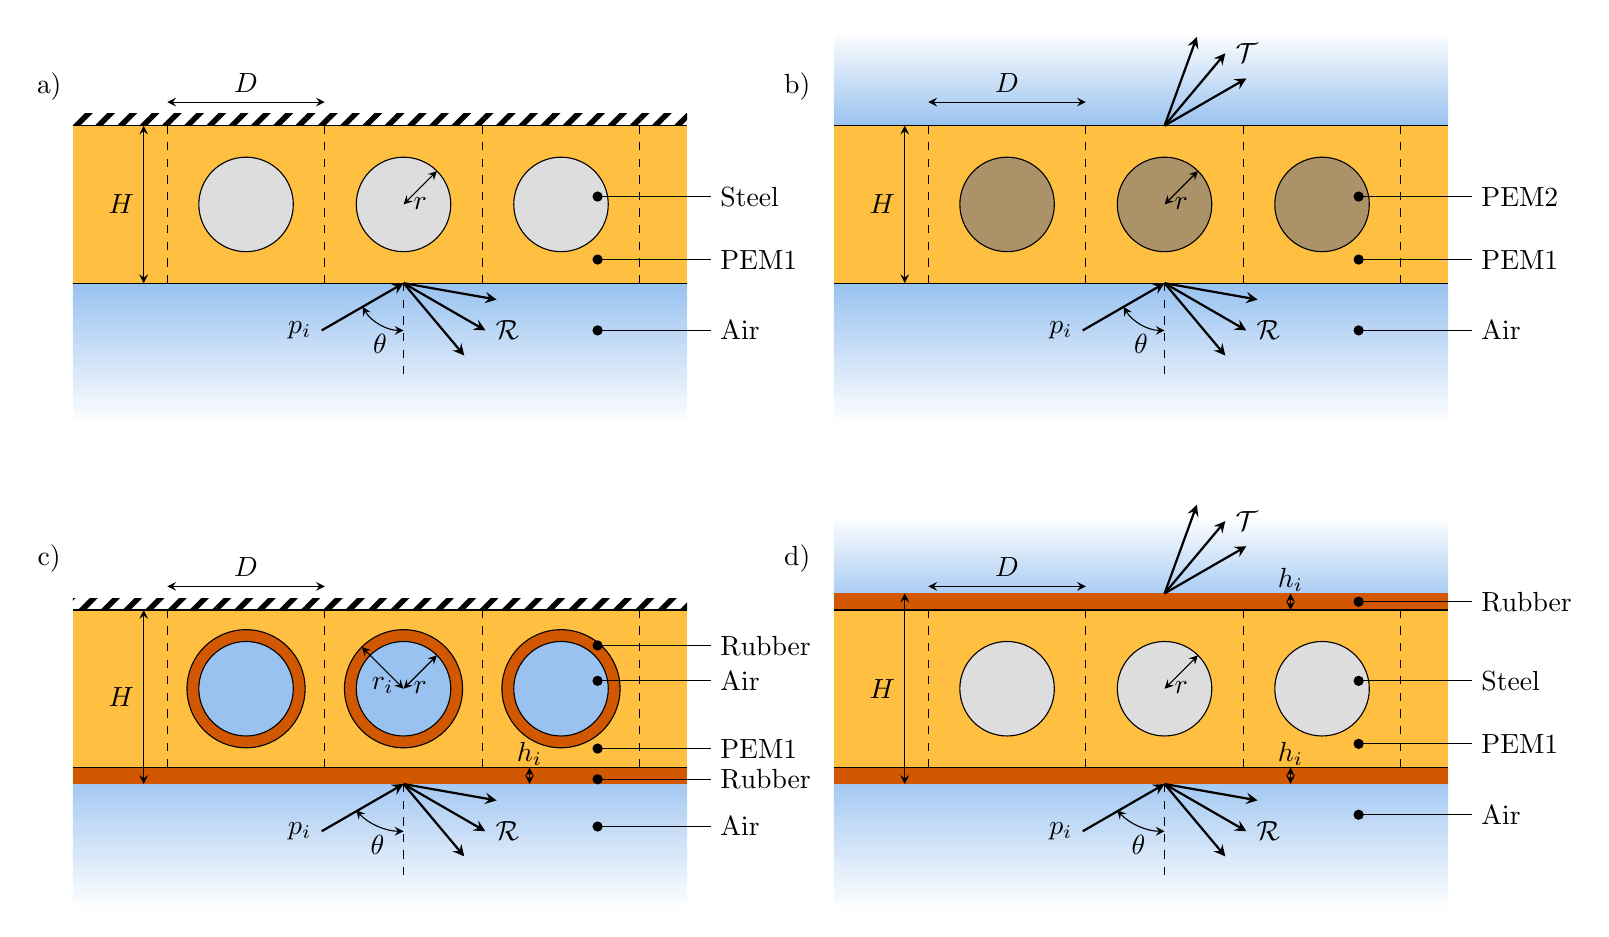
\begin{tikzpicture}

% Benchmark cas 1
\begin{scope}
    \def\cellen{2} \def\height{2} \def\pad{.3} \def\arrow{.7}\def\totalen{6}
    \fill [
           pattern={Lines[
                  distance=2mm,
                  angle=45,
                  line width=0.7mm
                 ]},
        pattern color=black
       ] (-4*\pad, \height) rectangle ++(\totalen+6*\pad, .5*\pad);
    \draw[top color = fluid, bottom color = white,draw=none] (-4*\pad, 0) rectangle ++ (\totalen+6*\pad, -6*\pad);
    \draw[fill=pem, draw=none] (-4*\pad, 0) rectangle ++ (\totalen+6*\pad, \height);

    \draw[black] (-4*\pad, 0) -- ++ (\totalen+6*\pad, 0);
    \draw[black] (-4*\pad, \height) -- ++ (\totalen+6*\pad, 0);
    \foreach \i in {0, 1, 2} {
        \draw[fill=steel] ((\i*\cellen + \cellen/2, \height/2) circle (2*\pad);
        \draw[dashed] (\i*\cellen, 0) -- ++ (0, \height);
        \draw[dashed] (\i*\cellen+\cellen, 0) -- ++ (0, \height);
        }
        
%    \draw[thick,->] (\cellen, 0) -- ++ (\arrow, 0) node[above] {$x_1$};
%    \draw[thick, ->] (\cellen, 0) -- ++ (0, \arrow) node[below right] {$x_2$};
    \draw[<->] (-\pad, 0) -- ++ (0, \height) node[midway, left] {$H$};
    \draw[<->] (0, \height+\pad) -- ++ (\cellen, 0) node[midway, above] {$D$};
    \draw[<->] (3*\cellen/2, \height/2) -- ++ (45:2*\pad) node[midway, below] {$r$};

    \draw[thick, <-] (3*\cellen/2, 0) -- ++ (210:4*\pad) node[left] {$p_i$};
    \draw[thick, ->] (3*\cellen/2, 0) -- ++ (-30:4*\pad) node[right] {$\mathcal R$};
    \draw[thick, ->] (3*\cellen/2, 0) -- ++ (-50:4*\pad);
    \draw[thick, ->] (3*\cellen/2, 0) -- ++ (-10:4*\pad);
    \draw[dashed] (3*\cellen/2, 0) -- ++ (0, -4*\pad);
    \draw[<->] (3*\cellen/2, -2*\pad) arc (90:30:-2*\pad) node[midway, below] {$\theta$};

    \draw[Circle-] (3*\cellen-2*\pad, \height-3*\pad) -- ++ (5*\pad, 0) node[right] {Steel};
    \draw[Circle-] (3*\cellen-2*\pad, \pad) -- ++ (5*\pad, 0) node[right] {PEM1};
    \draw[Circle-] (3*\cellen-2*\pad, -2*\pad) -- ++ (5*\pad, 0) node[right] {Air};
\end{scope}
% Benchmark cas 7
\begin{scope}[xshift=275]
    \def\cellen{2} \def\height{2} \def\pad{.3} \def\arrow{.7}\def\totalen{6}
    \draw[top color = white, bottom color=fluid, draw=none] (-4*\pad, \height) rectangle ++ (\totalen+6*\pad, 4*\pad);
    \draw[top color = fluid, bottom color = white,draw=none] (-4*\pad, 0) rectangle ++ (\totalen+6*\pad, -6*\pad);
    \draw[fill=pem, draw=none] (-4*\pad, 0) rectangle ++ (\totalen+6*\pad, \height);

    \draw[black] (-4*\pad, 0) -- ++ (\totalen+6*\pad, 0);
    \draw[black] (-4*\pad, \height) -- ++ (\totalen+6*\pad, 0);
    \foreach \i in {0, 1, 2} {
        \draw[fill=pem2] ((\i*\cellen + \cellen/2, \height/2) circle (2*\pad);
        \draw[dashed] (\i*\cellen, 0) -- ++ (0, \height);
        \draw[dashed] (\i*\cellen+\cellen, 0) -- ++ (0, \height);
        }
        
    %\draw[thick,->] (\cellen, 0) -- ++ (\arrow, 0) node[above] {$x_1$};
    %\draw[thick, ->] (\cellen, 0) -- ++ (0, \arrow) node[below right] {$x_2$};
    \draw[<->] (-\pad, 0) -- ++ (0, \height) node[midway, left] {$H$};
    \draw[<->] (0, \height+\pad) -- ++ (\cellen, 0) node[midway, above] {$D$};
    \draw[<->] (3*\cellen/2, \height/2) -- ++ (45:2*\pad) node[midway, below] {$r$};

    \draw[thick, ->] (3*\cellen/2, \height) -- ++ (50:4*\pad) node[right] {$\mathcal T$};
    \draw[thick, ->] (3*\cellen/2, \height) -- ++ (30:4*\pad) node[right] {};
    \draw[thick, ->] (3*\cellen/2, \height) -- ++ (70:4*\pad) node[right] {};
    \draw[thick, <-] (3*\cellen/2, 0) -- ++ (210:4*\pad) node[left] {$p_i$};
    \draw[thick, ->] (3*\cellen/2, 0) -- ++ (-30:4*\pad) node[right] {$\mathcal R$};
    \draw[thick, ->] (3*\cellen/2, 0) -- ++ (-50:4*\pad);
    \draw[thick, ->] (3*\cellen/2, 0) -- ++ (-10:4*\pad);
    \draw[dashed] (3*\cellen/2, 0) -- ++ (0, -4*\pad);
    \draw[<->] (3*\cellen/2, -2*\pad) arc (90:30:-2*\pad) node[midway, below] {$\theta$};

    \draw[Circle-] (3*\cellen-2*\pad, \height-3*\pad) -- ++ (5*\pad, 0) node[right] {PEM2};
    \draw[Circle-] (3*\cellen-2*\pad, \pad) -- ++ (5*\pad, 0) node[right] {PEM1};
    \draw[Circle-] (3*\cellen-2*\pad, -2*\pad) -- ++ (5*\pad, 0) node[right] {Air};
\end{scope}
% Benchmark cas 10
\begin{scope}[yshift=-175]
    \def\cellen{2} \def\height{2} \def\pad{.3} \def\arrow{.7}\def\totalen{6}
        \def\rubberthick{.7*\pad}

    \fill [
           pattern={Lines[
                  distance=2mm,
                  angle=45,
                  line width=0.7mm
                 ]},
        pattern color=black
       ] (-4*\pad, \height) rectangle ++(\totalen+6*\pad, .5*\pad);
    \draw[top color = fluid, bottom color = white,draw=none] (-4*\pad, 0) rectangle ++ (\totalen+6*\pad, -6*\pad);
    \draw[fill=pem, draw=none] (-4*\pad, 0) rectangle ++ (\totalen+6*\pad, \height);
    \draw[fill=rubber, draw=none] (-4*\pad, 0) rectangle ++ (\totalen+6*\pad, -\rubberthick);


    \draw[black] (-4*\pad, 0) -- ++ (\totalen+6*\pad, 0);
    \draw[black] (-4*\pad, \height) -- ++ (\totalen+6*\pad, 0);
    \foreach \i in {0, 1, 2} {
        \draw[fill=rubber] ((\i*\cellen + \cellen/2, \height/2) circle (2.5*\pad);
        \draw[fill=fluid] ((\i*\cellen + \cellen/2, \height/2) circle (2*\pad);
        \draw[dashed] (\i*\cellen, 0) -- ++ (0, \height);
        \draw[dashed] (\i*\cellen+\cellen, 0) -- ++ (0, \height);
        }
        
    %\draw[thick,->] (\cellen, 0) -- ++ (\arrow, 0) node[above] {$x_1$};
    %\draw[thick, ->] (\cellen, 0) -- ++ (0, \arrow) node[below right] {$x_2$};
    \draw[<->] (-\pad, -\rubberthick) -- ++ (0, \height+\rubberthick) node[midway, left] {$H$};
    \draw[<->] (0, \height+\pad) -- ++ (\cellen, 0) node[midway, above] {$D$};
    \draw[<->] (3*\cellen/2, \height/2) -- ++ (45:2*\pad) node[midway, below] {$r$};
    \draw[<->] (3*\cellen/2, \height/2) -- ++ (135:2.5*\pad) node[midway, below] {$r_i$};

    \draw[thick, <-] (3*\cellen/2, -\rubberthick) -- ++ (210:4*\pad) node[left] {$p_i$};
    \draw[thick, ->] (3*\cellen/2, -\rubberthick) -- ++ (-30:4*\pad) node[right] {$\mathcal R$};
    \draw[thick, ->] (3*\cellen/2, -\rubberthick) -- ++ (-50:4*\pad);
    \draw[thick, ->] (3*\cellen/2, -\rubberthick) -- ++ (-10:4*\pad);
    \draw[dashed] (3*\cellen/2, -\rubberthick) -- ++ (0, -4*\pad);
    \draw[<->] (3*\cellen/2, -2*\pad-\rubberthick) arc (90:42:-2*\pad-\rubberthick) node[midway, below] {$\theta$};
    \draw[<->] (2*\cellen+2*\pad, 0) -- ++ (0, -\rubberthick) node[midway, above] {$h_i$};

    \draw[Circle-] (3*\cellen-2*\pad, \height-1.5*\pad) -- ++ (5*\pad, 0) node[right] {Rubber};
    \draw[Circle-] (3*\cellen-2*\pad, \height-3*\pad) -- ++ (5*\pad, 0) node[right] {Air};
    \draw[Circle-] (3*\cellen-2*\pad, .8*\pad) -- ++ (5*\pad, 0) node[right] {PEM1};
    \draw[Circle-] (3*\cellen-2*\pad, -.15) -- ++ (5*\pad, 0) node[right] {Rubber};
    \draw[Circle-] (3*\cellen-2*\pad, -2.5*\pad) -- ++ (5*\pad, 0) node[right] {Air};
\end{scope}

% Benchmark cas 13
\begin{scope}[xshift=275, yshift=-175]
    \def\cellen{2} \def\height{2} \def\pad{.3} \def\arrow{.7}\def\totalen{6}
    \def\rubberthick{.7*\pad}
    \draw[top color = white, bottom color=fluid, draw=none] (-4*\pad, \height) rectangle ++ (\totalen+6*\pad, 4*\pad);
    \draw[top color = fluid, bottom color = white,draw=none] (-4*\pad, 0) rectangle ++ (\totalen+6*\pad, -6*\pad);
    \draw[fill=pem, draw=none] (-4*\pad, 0) rectangle ++ (\totalen+6*\pad, \height);
    \draw[fill=rubber, draw=none] (-4*\pad, \height) rectangle ++ (\totalen+6*\pad, \rubberthick);
    \draw[fill=rubber, draw=none] (-4*\pad, 0) rectangle ++ (\totalen+6*\pad, -\rubberthick);

    \draw[black] (-4*\pad, 0) -- ++ (\totalen+6*\pad, 0);
    \draw[black] (-4*\pad, \height) -- ++ (\totalen+6*\pad, 0);
    \foreach \i in {0, 1, 2} {
        \draw[fill=steel] ((\i*\cellen + \cellen/2, \height/2) circle (2*\pad);
        \draw[dashed] (\i*\cellen, 0) -- ++ (0, \height);
        \draw[dashed] (\i*\cellen+\cellen, 0) -- ++ (0, \height);
        }
        
    %\draw[thick,->] (\cellen, 0) -- ++ (\arrow, 0) node[above] {$x_1$};
    %\draw[thick, ->] (\cellen, 0) -- ++ (0, \arrow) node[below right] {$x_2$};
    \draw[<->] (-\pad, -\rubberthick) -- ++ (0, \height+2*\rubberthick) node[midway, left] {$H$};
    \draw[<->] (0, \height+\pad) -- ++ (\cellen, 0) node[midway, above] {$D$};
    \draw[<->] (2*\cellen+2*\pad, \height) -- ++ (0, \rubberthick) node[midway, above] {$h_i$};
    \draw[<->] (2*\cellen+2*\pad, 0) -- ++ (0, -\rubberthick) node[midway, above] {$h_i$};
    \draw[<->] (3*\cellen/2, \height/2) -- ++ (45:2*\pad) node[midway, below] {$r$};

    \draw[thick, ->] (3*\cellen/2, \height+\rubberthick) -- ++ (50:4*\pad) node[right] {$\mathcal T$};
    \draw[thick, ->] (3*\cellen/2, \height+\rubberthick) -- ++ (30:4*\pad) node[right] {};
    \draw[thick, ->] (3*\cellen/2, \height+\rubberthick) -- ++ (70:4*\pad) node[right] {};
    \draw[thick, <-] (3*\cellen/2, -\rubberthick) -- ++ (210:4*\pad) node[left] {$p_i$};
    \draw[thick, ->] (3*\cellen/2, -\rubberthick) -- ++ (-30:4*\pad) node[right] {$\mathcal R$};
    \draw[thick, ->] (3*\cellen/2, -\rubberthick) -- ++ (-50:4*\pad);
    \draw[thick, ->] (3*\cellen/2, -\rubberthick) -- ++ (-10:4*\pad);
    \draw[dashed] (3*\cellen/2, -\rubberthick) -- ++ (0, -4*\pad);
    \draw[<->] (3*\cellen/2, -2*\pad-\rubberthick) arc (90:42:-2*\pad-\rubberthick) node[midway, below] {$\theta$};

    \draw[Circle-] (3*\cellen-2*\pad, \height+\rubberthick/2) -- ++ (5*\pad, 0) node[right] {Rubber};
    \draw[Circle-] (3*\cellen-2*\pad, \height-3*\pad) -- ++ (5*\pad, 0) node[right] {Steel};
    \draw[Circle-] (3*\cellen-2*\pad, \pad) -- ++ (5*\pad, 0) node[right] {PEM1};
    \draw[Circle-] (3*\cellen-2*\pad, -2*\pad) -- ++ (5*\pad, 0) node[right] {Air};
\end{scope} 

\node at (-1.5, 2.5) {a)};
\node at (8, 2.5) {b)};
\node at (-1.5, -3.5) {c)};
\node at (8, -3.5) {d)};
\end{tikzpicture}
\end{document}

